\documentclass[a4paper]{article}

% Includes packages relevant to Senior Lab

% character set specifications
\usepackage[english]{babel}
\usepackage[utf8]{inputenc}

% increased vertical spacing for tables
\newcommand\topVspace{\rule{0pt}{2.6ex}}      
\newcommand\bottomVspace{\rule[-1.2ex]{0pt}{0pt}} 

% extra unicode characters
\DeclareUnicodeCharacter{3BC}{\(\mu\)}
\DeclareUnicodeCharacter{3C1}{\(\rho\)}
\DeclareUnicodeCharacter{2080}{\(_0\)}
\DeclareUnicodeCharacter{2081}{\(_1\)}
\DeclareUnicodeCharacter{2082}{\(_2\)}
\DeclareUnicodeCharacter{3B5}{\(\epsilon\)}
\DeclareUnicodeCharacter{3B1}{\(\alpha\)}

% SI Units
\usepackage{siunitx}

% extra SI units
\DeclareSIUnit\gauss{G}

% enable scientific notation
\sisetup{scientific-notation = engineering, exponent-to-prefix}

% draw pretty lines
\usepackage{tikz}
\usetikzlibrary{datavisualization}
\usepackage{circuitikz}

% manual tabbing
\setlength{\parindent}{0pt}
\def\qq{\qquad}

% include graphics
\usepackage{graphicx}

% increased control over figure placement
\usepackage{float}

% box answers
\usepackage{tcolorbox}

% enable multiple section levels
\usepackage{titlesec}

% define `\subsubsubsection` command
\titleclass{\subsubsubsection}{straight}[\subsection]
\newcounter{subsubsubsection}[subsubsection]
\renewcommand\thesubsubsubsection{\thesubsubsection.\arabic{subsubsubsection}}
\titleformat{\subsubsubsection}
        {\normalfont\normalsize\bfseries}{\thesubsubsubsection}{1em}{}
\titlespacing*{\subsubsubsection}
{0pt}{3.25ex plus 1ex minus .2ex}{1.5ex plus .2ex}
\setcounter{secnumdepth}{4}

% get align environment (among other things)
\usepackage{amsmath}

% bold in math mode
\usepackage{bm}

% get \mathbb (among other things)
\usepackage{amssymb}

\usepackage{array}

% plotting
\usepackage{pgfplots}

% enable external references
\usepackage{hyperref}

% include code
\usepackage[cache=false]{minted}
\setminted{linenos, frame=lines, texcomments}

% adjust margins of individual pages (for shoving figures into place)
\usepackage{changepage}

% rotate figures
\usepackage{rotating}


\usepackage{caption}
\renewcommand{\thetable}{\arabic{section}.\arabic{table}}
\newcommand\T{\rule{0pt}{2.6ex}}       % Top strut
\newcommand\B{\rule[-1.2ex]{0pt}{0pt}} % Bottom strut

\title{PHY 4210-01 Senior Lab \\Lab P2: Electron Spin Resonance}

\author{Sarah Arends \\
        Jacquelyne Miksanek \\
        Ryan Wojtyla \\ \\
        Instructor: Jerry Collins}

\date{March 28, 2019}

\begin{document}
\maketitle

\begin{abstract}
%physics of experiment
%apparatus used
%what was measured
%Results

\qq The Lande factor, $g_s$, (or the gyromagnetic ratio of spin) for the
electron was determined through the use of electron spin resonance and
Helmholtz coils. The g-factor of a diphenyl-picryl-hydrazyl (DPPH) sample was
obtained following the measurement of the frequency dependence of the
resonance field. The line width of the resonance signal was then calculated.

\end{abstract}

\newpage

\tableofcontents

\newpage

%Labeled sketch of the experimental setup
\begin{figure}[H]
\centering
% uncomment the line below to add image
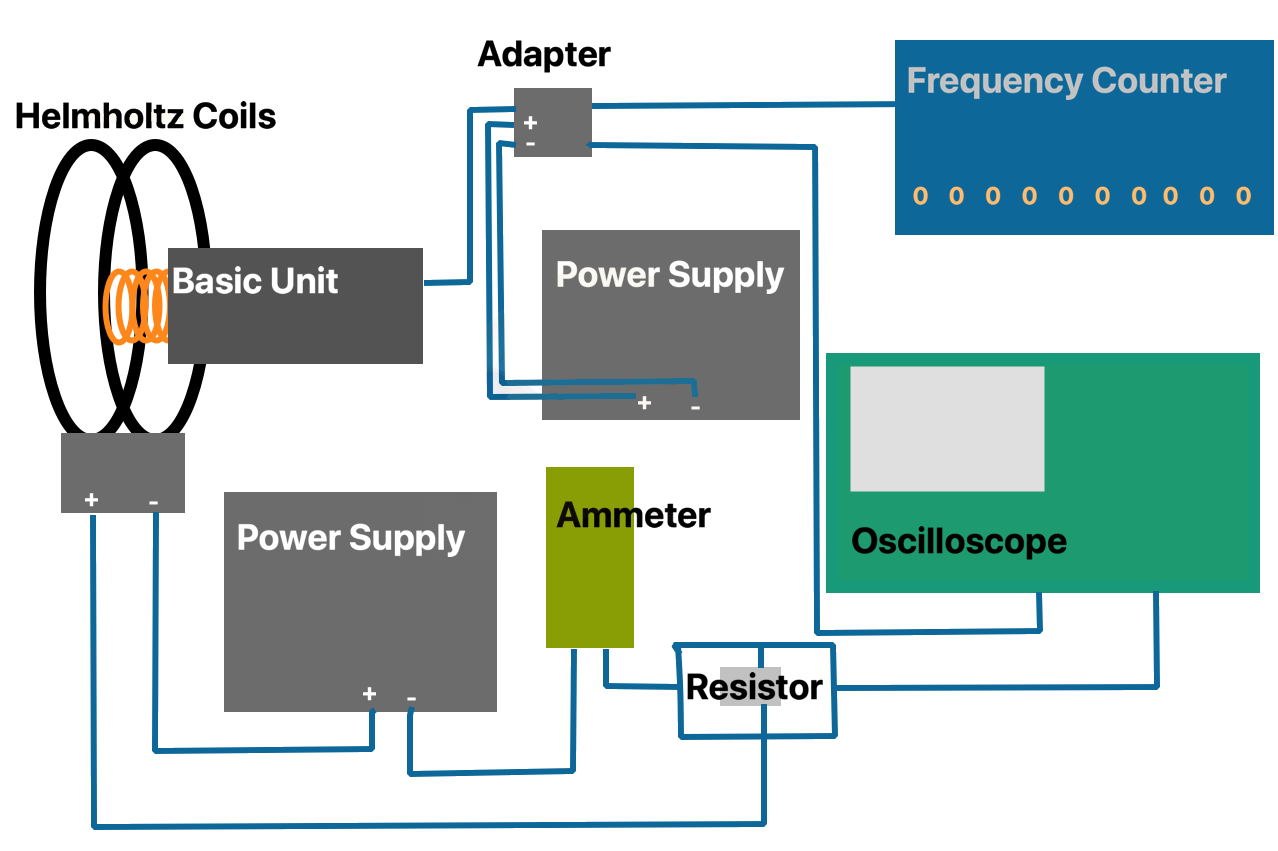
\includegraphics[width=1\textwidth]{Circuit_Diagram_P2Lab.png}
\captionof{figure}{Schematic of equipment used in experiment}
\label{Circuit_Diagram}
\end{figure}

\section{Data Analysis}
%Graphs, figures, and tables with captions
%Results with error analysis
%Calculate discrepancies from theory

\subsection{Frequency Dependence of Resonance Field}

\qq Voltage was compared to frequency to obtain a graphical
relationship for the frequency dependence of the resonance field. The
amplitude voltage was obtained by measuring the peak-to-peak voltage
from the oscilloscope and dividing it in half. The peak of
\ref{FrequencyDependece} is the specific resonance frequency for the
field. This value is a voltage amplitude of 1.01 V and a frequency of
$4.18*10^7$ Hz. It is important to note that the electron spin
resonance device divides the frequency by a factor of a thousand, and
thus the Hewlett-Packard frequency counter displayed a corrected
frequency. The calculations require an uncorrected frequency, i.e. the
counter's frequency multiplied by one thousand.
\begin{figure}[H]
\centering
% uncomment the line below to add image
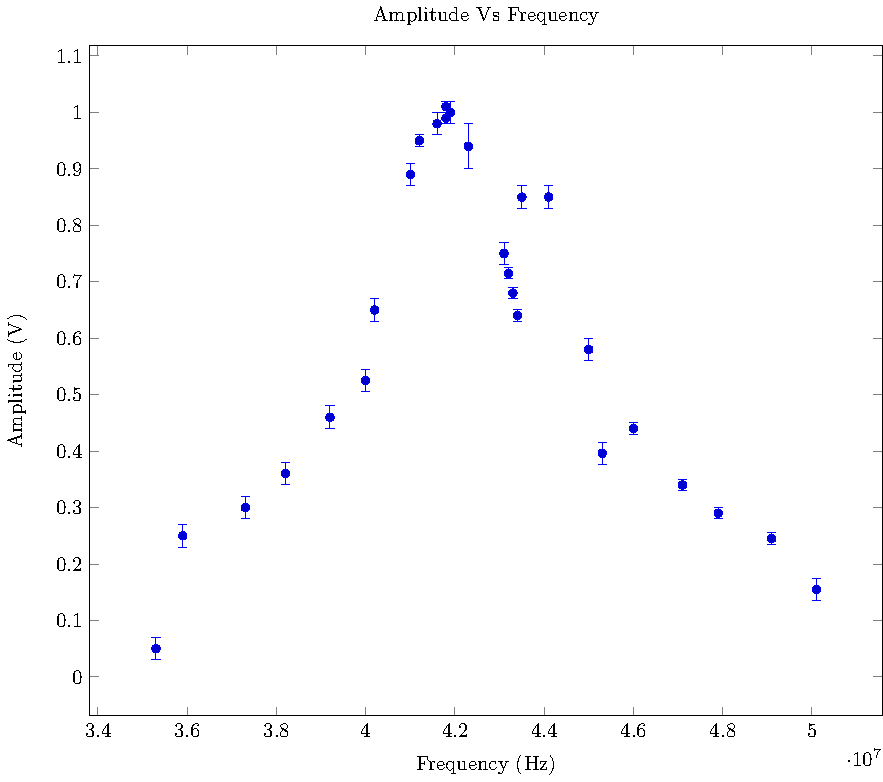
\includegraphics[scale=1.0]{Plots/ExpFreqVsVolt/freq_depen.pdf}
\captionof{figure}{Graphic representation of the frequency dependence
  of the resonance field.}
\label{FrequencyDependence}
\end{figure}

\subsection{Propagation of Uncertainty in the Frequency Dependence of the Resonance Field}

\subsection{Experimental Value of Gyromagnetic Ratio}
\qq The gyromagnetic ratio is calculated using the following equation,
where $\nu$ is the frequency, $h$ is Planck's constant, $\mu_B$ is the
Bohr magneton, and $B_0$ is the magnetic field strength.
\begin{equation}
\label{eq:exp_gs}
g_s = \frac{h \times \nu}{\mu_B \times B_0}
\end{equation}

\qq The magnetic field used in calculating equation \ref{eq:exp_gs}
must be calculated as well. It is determined from the measured current
using equation \ref{eq:exp_B}, where $\mu_0 = 4 \pi \times 10^{-7}
\frac{Vs}{Am}$, the number of turns is $n=320$, and the radius of the
coils is $r=6.8cm$.
\begin{equation}
\label{eq:exp_B}
B_0 = \mu_0 \left( \frac{4}{5} \right) ^{3/2} \times \frac{n}{r} \times I
\end{equation}

\qq Rather than measuring the current directly, the current is
calculated by measuring the voltage drop across a resistor, of which
the resistance is also measured. This calculation is shown below in
equation.
\begin{equation}
\label{eq:exp_I}
I = \frac{V}{R}
\end{equation}

\qq By substituting equation \ref{eq:exp_I} into \ref{eq:exp_B}, and
then substituting equation \ref{eq:exp_B} into equation
\ref{eq:exp_gs}, we arrive at an expression for the gyromagnetic ratio
in terms of known constants and measured quantities. This final
expression is shown in equation \ref{eq:exp_gs_combined}.
\begin{equation}
\label{eq:exp_gs_combined}
g_s = \frac{h \times \nu}{\mu_B \times \left( \mu_0 \left( \frac{4}{5}
  \right) ^{3/2} \times \frac{n}{r} \times \frac{V}{R} \right) }
\end{equation}

\subsection{Propagating Uncertainty in Gyromagnetic Ratio}
\qq The error in the experimental value of the gyromagnetic ratio is
determined by propagating uncertainty in equation
\ref{eq:exp_gs_combined}. There are no uncertainties associated with
fundamental constants such as $h$, $\mu_B$, and $\mu_0$. It is assumed
that the number of coil turns, $n$, also has no associated uncertainty
because it was reported in the manual as such. The uncertainty in the
radius is constant for all measurements, but the frequency, voltage,
and resistance will differ for each measurement. Equation
\ref{eq:delta_gs} shows this error propagation.

\begin{equation}
\label{eq:delta_gs}
\delta g_s = g_s \times
              \sqrt {
              		  \left( \frac{\delta \nu}{\nu} \right) ^2
              		+ \left( \frac{\delta r}{r} \right) ^2
              		+ \left( \frac{\delta V}{V} \right) ^2
              		+ \left( \frac{\delta R}{R} \right) ^2
					} \\
\end{equation}

An example calculation for the value of $g_s$ and its propagated
uncertainty is shown below for a measurement taken with the large
coil:

\begin{align*}
g_s &= \frac
		{6.626 \times 10^{-34} \times  \left( 3 \times 10^7 \right) }
		{\mu_B \times \left( 4 \pi \times 10^{-7}
						     \left( \frac{4}{5} \right) ^{3/2}
						     \times \frac{320}{0.068}
						     \times \frac{0.44}{1.7} \right)
	     } \\
    &= 1.93 \\
\end{align*}

\begin{align*}
\delta g_s &=
		   g_s \times
              \sqrt {
              		  \left( \frac{1.00 \times 10^4 \text{Hz}}{3.00 \times 10^7 \text{Hz}} \right) ^2
              		+ \left( \frac{0.5 \text{cm}}{6.7 \text{cm}} \right) ^2
              		+ \left( \frac{0.1 \text{V}}{2 \text{V}} \right) ^2
              		+ \left( \frac{0.1 \Omega}{1.7 \Omega} \right) ^2
					} \\
		  &= 1.93 \times
              \sqrt {
              		  \left( 3.3 \times 10^{-4} \right) ^2
              		+ \left( 0.006 \right) ^2
              		+ \left( 0.05 \right) ^2
              		+ \left( 0.06 \right) ^2
					} \\
		  &= .15
\end{align*}

We can calculate the discrepancy between the experimental and
theoretical values as follows. Recall the theoretical value of $g_s$
for DPPH is 2.0036, which is approximated as 2.00 due to the limited
precision of the experimental value.


\begin{align*}
\Delta g_s &= | g_{s_{exp}} - g_{s_{theo}} | \\ &= | 1.93 - 2.00 |
\\ &= 0.074 \\
\end{align*}

Evidently, this difference $\Delta g_s$ is less than $1 \sigma = .15$.

\subsection{Rejection of Data}
\qq During the data taking process for the "big coil", a measurement
at a particular frequency produced an experimental $g_s$ value that
seemed anomalous; most measurements fall between 1 and 4, but this
measurement is around 13. Chauvenet's criterion will be used to
determine if this datum should be discarded.

\qq If one assumes this measurement to be valid, the resultant average
and standard deviation are $2.59 \pm 2.91$ (quite an atrocity). The
measurement in question, 13.08, differs from the average by $4.49
\sigma$. If a Gaussian distribution is assumed for the $g_s$ values,
the probability of obtaining a measurement that differs from the mean
by this quantity is determined as follows:

\begin{align*}
Prob(\text{outside }  4.49 \sigma) &= 1 - Prob(\text{within } 4.49 \sigma) \\
							  &= 1 -  .9999994 \\
							  &= 0 \\
\end{align*}

\qq Since the probability of a measurement being withing $4.49 \sigma$
is so high, the probability of this measurement being outside this
interval is effectively zero. Therefore, we can discard the anomalous
datum with extremely high confidence.

\subsection{Determining Line Width of Resonance Signal}
\qq $\delta B_0$ is representative of an absorption line, and is
obtained when the energy is measured at a fixed frequency as function
of the magnetic field. The line width $\delta B_0$ is used as an
expression of the uncertainty in the energy of the transition. This is
best represented by the equation $\delta E = g \times \mu_0 \times
\delta B_0$. Using the uncertainty principle a relation is then found
for $\delta B_0$.

\begin{align*}
\delta B_0 = \frac{\hbar}{2 \times g_J \times \mu_B \times T}
\end{align*}
where T is the lifetime of the level and $g_J$ is the Land $\acute{e}$
factor. Experimentally $\delta B_0$ can be determined by the following equation:
\begin{align*}
\delta B_0 = B \times \left( \frac{\delta I}{I_{mod}} \right)
\end{align*}
where $\delta$I is represented as $\frac{\delta U}{U_{mod}} \times  I_{mod} \times 2\sqrt{2}$.

\begin{align*}
\delta I &= \frac{\delta U}{U_{mod}} \times  I_{mod} \times 2\sqrt{2} \\
         &= \frac{0.55}{2} \times 0.156 \times 2\sqrt{2} \\
         &= 0.121
\end{align*}

\begin{align*}
\delta B_0 &= B \times \left( \frac {\delta I} {I_{mod}} \right) \\
           &= 6.23 \times 10^{-4} \times \left( \frac {0.121} {0.156} \right) \\
           &= 4.85 \times 10^{-4} T \\
           &= 0.49 mT
\end{align*} 


\section{Results: Comparing Discrepancies and Uncertainties}
%Discuss results and uncertainties
%Compare results with theory
%Approximations to theory

\subsection{Discrepancy in Gyromagnetic Ratio}
\qq The discrepancy between the experimental and theoretical values of G for
each of the coils can be calculated with \( \Delta g_s = | g_{s_t} - g_{s_e} |
\), where \( g_{s_t} \) is the theoretical value of \( g_s \) and \( g_{s_e} \)
is the experimental value. The discrepancy in the value of \( g_s \) for the
small coil is:

\begin{align*}
  \Delta g_{s_{\text{small}}} =& \left| (2.00) - (1.44) \right| \\
  \Delta g_{s_{\text{small}}} =& 0.56 \\
\end{align*}

Since the standard deviation of the calculated values is
\( \sigma_{g_s, \text{small}} = 0.393 \), the experimental value of \( g_s \) is \(
\frac{\Delta g_{s_{\text{small}}}}{\sigma_{g_s, \text{small}}} = \frac{0.56}{0.393} = 1.42
\sigma \) from the theoretical value.

\qq The discrepancies for the medium and big coils were calculated in the same
way, and the results are detailed in Table \ref{tab:discrepancyG}.

\begin{table}[H]
  \caption{The discrepancies between the theoretical and experimental values for
    \( g_s \) for the small, medium, and big coils.}
  \begin{center}
    \begin{tabular}{|l|l|l|l|l|l|}
      \hline
      Coil & Theoretical \( g_s \) & Experimental \( g_s \) & \( \Delta g_s \) &
                                                                                 Standard
                                                                                 Deviation
                                                                                 (\(
                                                                                 \sigma
                                                                                 \)) &
                                                                                 \(
                                                                                 \sigma
                                                                                 \Delta
                                                                                 g_s
                                                                                 \)
      \\
      \hline
      Small & 2.00 & 1.44 & 0.56 & 0.393 & 1.42 \( \sigma \) \\
      Medium & 2.00 & 1.16 & 0.84 & 0.125 & 6.72 \( \sigma \) \\
      Big & 2.00 & 1.89 & 0.11 & 0.825 & 0.133 \( \sigma \) \\
      \hline
    \end{tabular}
  \end{center}
  \label{tab:discrepancyG}
\end{table}


\subsection{Discrepancy in Line Width}
\qq The line width itself is representative as an error in the energy,
as discussed above. Therefore, an uncertainty will not be calculated
in the line width, as it is already a calculation involving
uncertainties of constituent quantities. However, the experimental
value can be compared to an acceptable range given by literature
sources. The experimental line width was determined to be $\delta B_0
= 0.49 mT$. The range given for theoretical line width was [0.15,0.81]
mT, thus the experimental value is within the acceptable range.

\section{Sources of Error}
%Discuss the radius/seperation
%Discuss the equipment heating
\qq A true Helmholtz coil should have a separation distance equal to
that of the radius of the coil. The width of basic unit, which holds
the coil, was larger than the radius of the coil. Due to this the
separation was larger than the radius of the coil meaning that the
magnetic field is systematically lowered, as a true Helmhotz coil is
designed to maximize the constructive interference.  Furthermore,
because the magnetic field is systematically lower than the
prediction, the calculated $g_s$ is systematically raised in
value. Both the Helmholtz coil and the 1 $M \Omega$ resistor heated up
during the experimentation process. The heating of the equipment
causes the energy in the system to be systematically lowered as the
thermal energy transfers from the system to the surrounding region. This means
that the value of the $g_s$ is lowered compared to prediction. As the
resistor heats up the resistance changes, however this was accounted
for, and the resistance was remeasured for every trial and the
measured value was used in the calculations.

\section{Conclusion}
%Brief summary, discussion of results and theory
\qq

\section{Appendices}

\subsection{Appendix A: Data}

\subsection{Appendix B: Source Code}

\end{document}
